\chapter{Algorithme de segmentation}
Nous allons étudier le pseudo-code de cet algorithme qui nous est fourni.
\section{Question 1}
La boucle sur \textit{j} permet de parcourir tous les points au voisinage du point \textit{i} actuellement considéré. 

\section{Question 2}
Les distances sont en millimètres. Il convient dans cette question d'étudier trois constantes utilisées dans cet algorithme.
\begin{itemize}
  \item \textbf{\textit{k}} : il s'agit du \textbf{nombre de voisinage}, autrement dit le nombre de points autour d'un point considéré.\\\textit{Nous proposons la valeur \textbf{10}}.

\medskip

  \item \textbf{\textit{R}} : il s'agit de la \textbf{distance minimale} à laquelle on veut prendre en considération les points, par rapport au Lidar\\\textit{Nous proposons la valeur \textbf{10}}.

\medskip

  \item \textbf{\textit{D}} : il s'agit de la \textbf{distance maximale entre deux points} pour qu'ils soient considérés comme étant du même groupe\\\textit{Nous proposons la valeur \textbf{5}}.
\end{itemize}

\section{Question 3}
Une valeur constante pour le paramètre \textit{D} ne sera pas forcément adaptée à l'environnement dans lequel on évolue. Il faut donc la modifier en conséquence pour s'assurer que deux points appartenant réellement au même objet soient considérés comme tels dans notre module RTMaps.

\medskip

\textbf{La valeur de \textit{D} doit être proportionnelle à la distance du point considéré \textit{r[i]}.}

\section{Question 4}
La complexité de cet algorithme n'est pas forcément optimale (O(n\up{2})). De plus, l'usage de la constante \textit{D} n'est pas recommandé, comme vu à la question précédente. Cetains objets identifiés comme tels pourraient très bien être deux objets distincts.

\chapter{Développement}
\noindent Dans RTMaps, nous avons dû importer \textbf{wifibot\_sensors.pck} et \textbf{wifibot\_tools.pck} (trouvables dans \textit{D:/wifibot/Code/component\_package1}) avec comme paramètres :
\begin{itemize}
  \item mode : serial
  \item ip\_or\_com : COM12
  \item por\_or\_baudrate : 19200
  \item NbPoint : 680
\end{itemize}

\noindent Dans le \textit{Device manager} de Windows, il faut regarder sur quel port COM le Hokuyo est branché.

\section{Question 5}
Nous avons effectué la conversion des coordonnées polaires en coordonnées cartésiennes dans la fonction \textbf{readScanFromInput} comme suit :
\cpp
\begin{lstlisting}
void
ClusterComponent::readScanFromInput(std::vector<vec2d>& points)
{
  MAPSIOElt* angles    = StartReading(Input("Angles"));
  MAPSIOElt* distances = StartReading(Input("Distances"));
  if (angles->VectorSize() != distances->VectorSize())
    Error("angles/distances size mismatch");

  // Allocate enough memory to store the points.
  points.resize(angles->VectorSize());

  // Convert from scan space to 2D space.
  for (int i = 0; i < angles->VectorSize(); ++i)
  {
    points[i].x = distances->Integer32(i) * std::cos( angles->Float64(i) * M_PI / 180.0 );
    points[i].y = distances->Integer32(i) * std::sin( angles->Float64(i) * M_PI / 180.0 );
  }
}
\end{lstlisting}

Voici le résultat dans RTMaps du diagramme qui nous permet de tester notre module compilé :

\begin{figure}[!h]
   \centering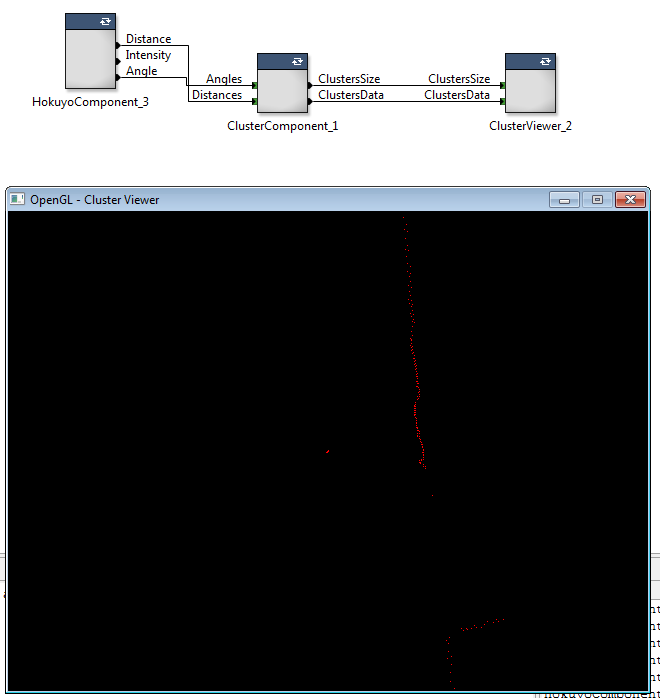
\includegraphics[width=0.85\textwidth]{question5.png}
   \caption{RTMaps}
\end{figure}

\newpage
\section{Question 6}
\subsection{Explication de la fonction \lstinline{sendClusters}}
\cpp
\begin{lstlisting}
void
ClusterComponent::sendClusters(std::vector<Cluster> const& clusters)
{
  // Sorties (il y en a 2)
  MAPSIOElt* clustersSize = StartWriting(Output("ClustersSize"));
  MAPSIOElt* clustersData = StartWriting(Output("ClustersData"));

  size_t nbPoints = 0; // Au départ il n'y a pas de point
  for (unsigned int i = 0; i < clusters.size(); ++i)
    nbPoints += clusters[i].size();
  // nbPoints = nbPoints + le nombre de points de chaque cluster

  // Allocation de la mémoire des buffers de sortie
  clustersSize->VectorSize() = clusters.size();
  clustersData->VectorSize() = nbPoints;

  unsigned int offset = 0;
  for (unsigned int i = 0; i < clusters.size(); ++i)
  {
    // On écrit la taille du cluster sur la sortie qui sert à ça
    clustersSize->Integer32(i) = clusters[i].size();

    // Pour chaque cluster on écrit ses points (coordonnées x et y)
    for (unsigned int j = 0; j < clusters[i].size(); ++j)
    {
      // Comme 'offset' est incrémenté à chaque passage, chaque point est écrit
      // successivement sur la sortie, en commençant par sa coordonnée x puis y
      // Par exemple avec des points de 1 à n : 1.x, 1.y, 2.x, 2.y, 3.x, ..., n.y
      clustersData->Float64(offset++) = clusters[i][j].x;
      clustersData->Float64(offset++) = clusters[i][j].y;
    }
  }

  StopWriting(clustersSize);
  StopWriting(clustersData);
}
\end{lstlisting}

\subsection{Fonction \lstinline{computerClusters}}
Voici la fonction \textbf{computerClusters} implémentée à partir du pseudo-code fourni dans le suejt du TP :
\cpp
\begin{lstlisting}
/*
 * points : Points d'entrée
 * clusters : tableau de cluster en sortie de l'algorithme
 */
void
sy31::computeClusters(std::vector<sy31::Cluster>& clusters, std::vector<sy31::vec2d> const& points)
{
  // Exemple d'utilisation des clusters
  //clusters.clear();    // Effacer tout les clusters
  //clusters.resize(1);    // Créer un cluster
  //clusters[0].clear(); // Effacer le cluster 0 (Initialiser)

  // Initialisations
  int *G=new int[points.size()]; // tableau G, groupes
  double d[K]={0}; // tableau D, distance
  int g=0; // aucun groupe
  for(int i=0; i<(int)points.size(); ++i)
  {
    clusters[0].push_back(points[i]); // Rajoute le point à la fin de clusters[]
    G[i]=0;
  }

  // Début de l'algo
  for(int i=K;i<=(int)points.size();i++)
  {
    double dmin=100;
    int jmin;
    if(sqrt(pow(points[i].x,2)+pow(points[i].y,2))>R)
    {
      for(int j=1;j<=K;j++)
      {
        d[j]=sqrt(pow(points[i].x-points[i-j].x,2)+pow(points[i].y-points[i-j].y,2));
        if(d[j]<dmin)
        {
          dmin=d[j];
          jmin=j;
        }
      }
    }

    if(dmin<D)
    {
      if(G[i-jmin]==0)
      {
        g++;
        G[i-jmin]=g;
        clusters.resize(g);
        clusters[G[i-jmin]-1].push_back(points[i-jmin]);
      }
      G[i]=G[i-jmin];
      clusters[G[i]-1].push_back(points[i]);
    }
  }
}
\end{lstlisting}

\section{Question 7}

Pour pouvoir filtrer les groupes dont le nombre de points est inférieur à un seuil \textit{N\textsubscript{min}}, il faut modifier la fonction \lstinline{sendClusters} comme ceci :

\cpp
\begin{lstlisting}
void ClusterComponent::sendClusters(std::vector<Cluster> const& clusters)
{
  // [...]
  unsigned int offset = 0;
  for (unsigned int i = 0; i < clusters.size(); ++i)
  {
    if (clusters.size() < Nmin) continue; // CETTE LIGNE FILTRE
  // [...]
\end{lstlisting}
La constante \textit{Nmin} pourrait être définie en tant que constante dans les fichiers d'en-tête, ou être un paramètre de la fonction \lstinline{sendClusters}.

\section{Question 8}

Faute de temps, nous n'avons pas pu essayer plusieurs paramètres afin de trouver ceux adéquats.

\medskip

L'algorithme s'avère être fonctionnel mais très imprécis. Nous avons eu du mal à identifier les objets nous entourant à l'écran.